\documentclass[]{beamer}
\usefonttheme{structurebold}
\usepackage{amssymb,amsmath}
\usepackage{ifxetex,ifluatex}
\usepackage{fixltx2e} % provides \textsubscript
\usepackage{lmodern}
\ifxetex
  \usepackage{fontspec,xltxtra,xunicode}
  \defaultfontfeatures{Mapping=tex-text,Scale=MatchLowercase}
  \newcommand{\euro}{€}
\else
  \ifluatex
    \usepackage{fontspec}
    \defaultfontfeatures{Mapping=tex-text,Scale=MatchLowercase}
    \newcommand{\euro}{€}
  \else
    \usepackage[T1]{fontenc}
    \usepackage[utf8]{inputenc}
      \fi
\fi
\IfFileExists{upquote.sty}{\usepackage{upquote}}{}
% use microtype if available
\IfFileExists{microtype.sty}{\usepackage{microtype}}{}
\usepackage{longtable,booktabs}
\usepackage{caption}
% These lines are needed to make table captions work with longtable:
\makeatletter
\def\fnum@table{\tablename~\thetable}
\makeatother
\usepackage{letltxmacro}
\LetLtxMacro\latexincludegraphics\includegraphics
\renewcommand{\includegraphics}[2][]{%
\centering
 \latexincludegraphics[#1]{#2}
}
\providecommand{\tightlist}{%
  \setlength{\itemsep}{0pt}\setlength{\parskip}{0pt}}
% Comment these out if you don't want a slide with just the
% part/section/subsection/subsubsection title:
\AtBeginPart{
  \let\insertpartnumber\relax
  \let\partname\relax
  \frame{\partpage}
}
\AtBeginSection{
  \let\insertsectionnumber\relax
  \let\sectionname\relax
  \frame{\sectionpage}
}
\AtBeginSubsection{
  \let\insertsubsectionnumber\relax
  \let\subsectionname\relax
  \frame{\subsectionpage}
}

\setlength{\parindent}{0pt}
\setlength{\parskip}{6pt plus 2pt minus 1pt}
\setlength{\emergencystretch}{3em}  % prevent overfull lines
\setcounter{secnumdepth}{0}
% Macros
\newcommand{\RR}{\mathbb{R}}
\newcommand{\CC}{\mathbb{C}}
\newcommand{\TR}{\text{T}}
\newcommand{\CO}{\text{conv}}

% Theme
\setbeamertemplate{navigation symbols}{}
\setbeamercovered{transparent}

% Colors
\definecolor{MapleBlue}{RGB}{1, 134, 190}
\usecolortheme{orchid}
\setbeamercolor{title}{fg=black}
\setbeamercolor{author}{fg=MapleBlue}
\setbeamercolor{frametitle}{fg=white}
\setbeamercolor{block title}{fg=white, bg=MapleBlue}
  
% Fonts
\setbeamerfont{date}{size=\fontsize{8pt}{9pt}}
	
% Custom title page

\setbeamertemplate{title page}
{

    \bigskip
	\bigskip
    {\usebeamerfont{subtitle}\usebeamercolor[fg]{subtitle}\insertsubtitle}\par
    {\usebeamerfont{title}\usebeamercolor[fg]{title}\inserttitle}\par
    {\usebeamerfont{author}\usebeamercolor[fg]{author}\insertauthor}\par
    {\usebeamerfont{date}\usebeamercolor[fg]{date}\insertdate}\par

}

\usebackgroundtemplate{\includegraphics[height=\paperheight,width=\paperwidth]{img/MapleBackground.png}}

\title{Autonomous Race Cars}
\subtitle{Nonlinear Model Predictive Control for}
\author{Behzad Samadi}
\date{Research Group, Maplesoft, Waterloo}

\begin{document}
\frame{\titlepage}

\usebackgroundtemplate{\includegraphics[width=\paperwidth]{img/Slides.png}}

\begin{frame}{Autonomous Race Cars Are Here}

\begin{itemize}
\tightlist
\item
  Roborace will be a motorsport championship similar to the FIA Formula
  E Championship but with autonomously-driven electric race cars.
\end{itemize}

\begin{figure}[!htb]
\centering
\href{http://danielsimon.com/roborace-robocar/}{\includegraphics[width=0.79\textwidth]{img/Roborace_DanielSimon_Robocar_002.jpg}}
\url{http://danielsimon.com/roborace-robocar/}
\end{figure}

\end{frame}

\begin{frame}{Model Predictive Driver}

\begin{itemize}
\tightlist
\item
  A race driver needs to look forward! (\textbf{prediction})
\item
  Minimize a cost function at each time instant depending on the current
  situation (\textbf{closed loop optimal control})
\item
  Optimization constraints:

  \begin{itemize}
  \tightlist
  \item
    Vehicle's dynamic behavior
  \item
    Limited power
  \item
    No skidding
  \item
    Following the road
  \item
    Avoiding collision
  \end{itemize}
\end{itemize}

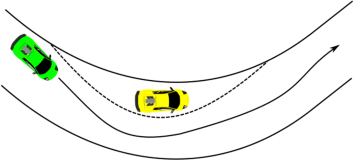
\includegraphics{img/MPCroad.pdf}

\end{frame}

\begin{frame}{Model Predictive Control}

\begin{itemize}
\tightlist
\item
  MPC is the optimal controller in the loop:

  \begin{enumerate}
  \def\labelenumi{\arabic{enumi}.}
  \tightlist
  \item
    Measure/estimate the current state \(x_n\).
  \item
    Solve the optimal control problem to compute \(u_k\) for
    \(k=n,\ldots,n+N-1\).
  \item
    Return \(u_n\) as the value of the control input.
  \item
    Update \(n\).
  \item
    Goto step 1.
  \end{enumerate}
\item
  MPC is implemented in real time.
\end{itemize}

\end{frame}

\begin{frame}{NMPC: Problem and Solution}

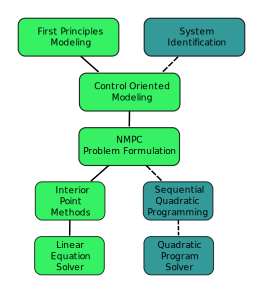
\includegraphics{img/NMPC_bigpic.pdf}

\end{frame}

\begin{frame}{Nonlinear Model}

\begin{itemize}
\tightlist
\item
  Consider the following nonlinear system:

  \begin{align*}
  \dot x(t)=&f(x(t),u(t))\\
  x(t_0)=&x_\circ
  \end{align*}

  where:

  \begin{itemize}
  \tightlist
  \item
    \(x(t)\) is the state vector
  \item
    \(u(t)\) is the input vector
  \end{itemize}
\end{itemize}

\end{frame}

\begin{frame}{Optimal Control Problem}

\begin{align*}
\underset{u}{\text{minimize}}\ & J(x_0,t_0)=\phi(x(t_f))+\int_{t_0}^{t_f}L(x(\tau),u(\tau))d\tau \\
\text{subject to} &\ \dot x(t)=f(x(t),u(t))\\
                  &\ x(t_0)=x_\circ\\
                  &\ g_i(x(t),u(t)) = 0, \text{ for }\ i=1,\ldots,n_g\\
                  &\ h_i(x(t),u(t)) \leq 0, \text{ for }\ i=1,\ldots,n_h
\end{align*}

\end{frame}

\begin{frame}{Discretization}

\begin{itemize}
\tightlist
\item
  Discretize the problem into \(N\) steps from \(t_0\) to \(t_f\):

  \begin{align*}
  \underset{u,\alpha}{\text{minimize}} &\ \phi_d(x_N)+\sum_{k=0}^{N-1}\left(L(x_k,u_k) \right)\\
  \text{subject to} &\ x_{k+1}=f_d(x_k,u_k)\\
                &\ x_0=x_\circ\\
                &\ g_i(x_k,u_k) = 0, \text{ for }\ i=1,\ldots,n_g\\
                &\ h_i(x_k,u_k) \leq 0, \text{ for }\ i=1,\ldots,n_h\\
  \end{align*}

  where \(\Delta\tau=\frac{t_f-t_0}{N}\) and:
  \[\phi_d(x_N)=\frac{\phi(x(t_f),t_f)}{\Delta\tau}\]
  \[f_d(x_k,u_k)=x_k+ f(x_k,u_k)\Delta\tau\]
\end{itemize}

\end{frame}

\begin{frame}{Interior Point - Barrier Method}

\begin{itemize}
\tightlist
\item
  Using a particular \emph{interior-point algorithm}, the \emph{barrier
  method}, the inequality constraints are converted to equality
  constraints:

  \begin{align*}
  \underset{u,\alpha}{\text{minimize}} &\ \phi_d(x_N)+\sum_{k=0}^{N-1}\left(L(x_k,u_k)-r^\text{T}\alpha_{k} \right)\\
  \text{subject to} &\ x_{k+1}=f_d(x_k,u_k)\\
                &\ x_0=x_\circ\\
                &\ g_i(x_k,u_k) = 0, \text{ for }\ i=1,\ldots,n_g\\
                &\ h_i(x_k,u_k) + \alpha_{ik}^2 = 0, \text{ for }\ i=1,\ldots,n_h\\
  \end{align*}

  where \(\alpha_k\in\mathbb{R}^{n_h}\) is a vector slack variable and
  the entries of \(r\in\mathbb{R}^{n_h}\) are small positive numbers.
\end{itemize}

(Boyd and Vandenberghe 2004)

\vspace{-2mm}

(Diehl, Ferreau, and Haverbeke 2009)

\end{frame}

\begin{frame}{Optimization Problem}

\begin{align*}
\underset{u,\alpha}{\text{minimize}} &\ \phi_d(x_N)+\sum_{k=0}^{N-1}\left(L(x_k,u_k)-r^\text{T}\alpha_{k} \right)\\
\text{subject to} &\ x_{k+1}=f_d(x_k,u_k)\\
                  &\ x_0=x_\circ\\
                  &\ G(x_k,u_k,\alpha_k) = 0
\end{align*}

where: \[ G(x_k,u_k,\alpha_k) = \left[\begin{array}{c}
                g_1(x_k,u_k)\\
                \vdots\\
                g_{n_g}(x_k,u_k)\\
                h_1(x_k,u_k) + \alpha_{1k}^2\\
                \vdots\\
                h_{n_h}(x_k,u_k) + \alpha_{n_hk}^2\\                
                \end{array}\right]\]

\end{frame}

\begin{frame}{Lagrange Multipliers}

\begin{itemize}
\tightlist
\item
  Lagrange multipliers: \vspace{-5mm}

  \begin{align*}
  \mathcal{L}(x,u,\alpha,\lambda,\nu)= &\ \phi_d(x_N,N)+ (x_\circ-x_0)^\text{T}\lambda_0\\
          &\ +\sum_{k=0}^{N-1}\left(L(x_k,u_k)-r^\text{T}\alpha_{k} \right.\\
          &\ +(f_d(x_k,u_k)-x_{k+1})^\text{T}\lambda_{k+1}\\
          &\ \left.+G(x_k,u_k,\alpha_k)^\text{T} \nu_{k} \right)
  \end{align*}
\item
  Optimality conditions:
  \[\mathcal{L}_{x_k}=0, \mathcal{L}_{\lambda_k}=0\ \text{for}\ k=0,\ldots,N \]
  \[\mathcal{L}_{\alpha_{k}}=0, \mathcal{L}_{u_k}=0, \mathcal{L}_{\nu_k}=0\ \text{for}\  k=0,\ldots,N-1\]
\end{itemize}

\end{frame}

\begin{frame}{Hamiltonian}

\begin{itemize}
\tightlist
\item
  \(\mathcal{L}(x,u,\alpha,\lambda,\nu)\) can be rewritten as:
  \vspace{-5mm}

  \begin{align*}
  \mathcal{L}(x,u,\alpha,\lambda,\nu)= &\phi_d(x_N)+x_\circ^\text{T}\lambda_0-x_N^\text{T}\lambda_N\\
          &\ +\sum_{k=0}^{N-1}\left(\mathcal{H}(x_k,u_k,\alpha_k,\lambda_{k+1})-x_{k}^\text{T}\lambda_k\right)
  \end{align*}
\item
  Hamiltonian:

  \begin{align*}
  \mathcal{H}(x_k,u_k,\alpha_k,\lambda_{k+1},\nu_k)=&L(x_k,u_k)-r^\text{T}\alpha_{k}\\
          &\ +f_d(x_k,u_k)^\text{T}\lambda_{k+1}+G(x_k,u_k,\alpha_k)^\text{T} \nu_{k}
  \end{align*}
\end{itemize}

\end{frame}

\begin{frame}{Pontryagin's Maximum Principle}

\begin{longtable}[]{@{}lc@{}}
\toprule
& Optimality Conditions\tabularnewline
\midrule
\endhead
\(\mathcal{L}_{\lambda_{k+1}}=0\) &
\(x_{k+1}^\star=f_d(x_k^\star,u_k^\star)\)\tabularnewline
\(\mathcal{L}_{\lambda_0}=0\) & \(x_0^\star=x_\circ\)\tabularnewline
\(\mathcal{L}_{x_k}=0\) &
\(\lambda_k^\star=\mathcal{H}_x(x_k^\star,u_k^\star,\alpha_k^\star,\lambda_{k+1}^\star,\nu_k^\star)\)\tabularnewline
\(\mathcal{L}_{x_N}=0\) &
\(\lambda_N^\star=\frac{\partial}{\partial x_N}\phi_d(x_N^\star)\)\tabularnewline
\(\mathcal{L}_{u_k}=0\) &
\(\mathcal{H}_u(x_k^\star,u_k^\star,\alpha_k^\star,\lambda_{k+1}^\star,\nu_k^\star)=0\)\tabularnewline
\(\mathcal{L}_{\alpha_k}=0\) &
\(\mathcal{H}_\alpha(x_k^\star,u_k^\star,\alpha_k^\star,\lambda_{k+1}^\star,\nu_k^\star)=0\)\tabularnewline
\(\mathcal{L}_{\nu_k}=0\) &
\(G(x_k^\star,u_k^\star,\alpha_k^\star) = 0\)\tabularnewline
\bottomrule
\end{longtable}

for \(k=0,\ldots,N-1\) where \(\star\) denote the optimal solution

\end{frame}

\begin{frame}{cGMRES Method: Compute Optimality Conditions}

\begin{itemize}
\tightlist
\item
  Step 1: Compute \(x_k\) and \(\lambda_k\) as functions of \(u_k\),
  \(\alpha_k\) and \(\nu_k\), given the following equations:

  \begin{align*}
  x_{k+1}=&\ f_d(x_k,u_k)\\
  x_0=&\ x_n\\
  \lambda_k=&\ \mathcal{H}_x(x_k,u_k,\alpha_k,\lambda_{k+1},\nu_k)\\
  \lambda_N=&\ \frac{\partial}{\partial x_N}\phi_d(x_N)
  \end{align*}
\end{itemize}

(Ohtsuka 2004)

\end{frame}

\begin{frame}{cGMRES Method: Compute Optimality Conditions}

\begin{itemize}
\tightlist
\item
  Step 2: For
  \[U=[u_0^\text{T},\ldots,u_{N-1}^\text{T},\alpha_0^\text{T},\ldots,\alpha_{N-1}^\text{T},\nu_0^\text{T},\ldots,\nu_{N-1}^\text{T}]^\text{T}\]
  solve the equation \(F(x_n, U)=0\), where: \[
  F(x_n, U)=\left[\begin{array}{c}
  \mathcal{H}_u(x_0,u_0,\alpha_0,\lambda_1,\nu_0)\\
  \mathcal{H}_\alpha(x_0,u_0,\alpha_0,\lambda_1,\nu_0)\\
  G(x_0,u_0,\alpha_0)\\
  \vdots\\
  \mathcal{H}_u(x_{N-1},u_{N-1},\alpha_{N-1},\lambda_N,\nu_{N-1})\\
  \mathcal{H}_\alpha(x_{N-1},u_{N-1},\alpha_{N-1},\lambda_N,\nu_{N-1})\\
  G(x_{N-1},u_{N-1},\alpha_{N-1})\\
  \end{array}\right]
  \]
\end{itemize}

(Ohtsuka 2004)

\end{frame}

\begin{frame}{cGMRES Method: Solver}

\begin{itemize}
\item
  \emph{Continuation method}: Instead of solving \(F(x, U)=0\), find
  \(U\) such that: \[\dot F(x, U)=A_sF(x, U)\] where \(A_s\) is a matrix
  with negative eigenvalues.
\item
  Now, we have: \[F_x\dot x+F_U\dot U=A_sF(x, U)\]
\item
  \emph{GMRES}: To compute \(\dot U\) using the following equation,
  which is linear in \(\dot U\), we use the generalized minimum residual
  (GMRES) algorithm. \[F_U\dot U=A_sF(x, U)-F_xf(x,u)\]
\item
  To compute \(U\) at any given time, we need to have an initial value
  for \(U\) and then use the above \(\dot U\) to update it.
\end{itemize}

(Ohtsuka 2004)

\end{frame}

\begin{frame}{cGMRES Method: Solver}

\begin{itemize}
\tightlist
\item
  \emph{Numerical approximation}:
  \[F_U\dot U\simeq \frac{F(x+hf(x,u),U+h\dot U)-F(x+hf(x,u),U)}{h}\]
  \[F_xf(x,u)\simeq\frac{F(x+hf(x,u),U)-F(x,U)}{h}\]
\end{itemize}

(Ohtsuka 2004)

\end{frame}

\begin{frame}{Maple Implementation}

\begin{itemize}
\tightlist
\item
  \emph{Problem formulation}:
  \[A(x,U,\dot U) = \frac{F(x,U+h\dot U)-F(x,U)}{h}\]
  \[b(x,U) = A_sF(x, U)-\frac{F(x+hf(x,u),U)-F(x,U)}{h}\]
\item
  \(b(x,U)\) is only called once per each step at the beginning and
  \(A(x,U,\dot U)\) is called several times by the GMRES solver.
\end{itemize}

\end{frame}

\begin{frame}{Maple Implementation}

\begin{itemize}
\tightlist
\item
  Maple procedures are generated for \(A\), \(b\) and optimized.
\item
  The GMRES solver is also implemented in Maple.
\item
  C code is then generated automatically.
\item
  The C code is then used to simulate the closed loop system in
  Maplesim.
\end{itemize}

\end{frame}

\begin{frame}{Interior Point Methods}

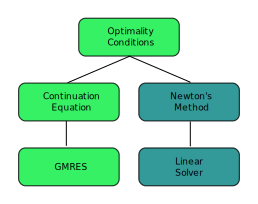
\includegraphics{img/cGMRES.pdf}

\end{frame}

\begin{frame}{Application: Autonomous Race Car}

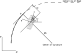
\includegraphics[width=3.33333in]{img/SpatialVehicleModel.pdf}

\vspace{-1cm}

\[\dot s=\frac{\rho_r}{\rho_r-y_r}(v_x\cos(\psi_e)-v_y\sin(\psi_e))\]

\end{frame}

\begin{frame}{Application: Autonomous Race Car}

\begin{block}{Approximate Vehicle Model}
\begin{align*}
\dot X &=v\cos(\psi+C_1\delta)\\
\dot Y &=v\sin(\psi+C_1\delta)\\
\dot \psi &= vC_2\delta\\
\dot v &= (C_{m_1}-C_{m_2}v)F_{x_r}-C_{r_2}v^2-C_{r_0}-(v\delta)^2C_2C_1
\end{align*}
\end{block}

(Verschueren et al. 2014)

\end{frame}

\begin{frame}{Application: Autonomous Race Car}

\begin{block}{Key Equation}
\[\frac{dz}{ds}=\frac{\dot z}{\dot s}\]
\end{block}

\begin{block}{Velocity on the Centerline}
\[\dot s = \frac{1}{1-\kappa_r y_r}(v_x\cos(\psi_e)-v_y\sin(\psi_e))\]
where:
\[\kappa_r=\frac{1}{\rho}\]
\end{block}

\end{frame}

\begin{frame}{Application: Autonomous Race Car}

\begin{block}{Spatial model}
\begin{align*}
\frac{dy_r}{ds}=&\frac{1}{\dot s} (v\sin(\psi)+vC_1\delta\cos(\psi))\\
\frac{d\psi_e}{ds}=&\frac{\dot \psi}{\dot s}-\kappa_r\\
\frac{dv}{ds}=&\frac{\dot v}{\dot s}\\
\frac{dt}{ds}=&\frac{1}{\dot s}
\end{align*}
\end{block}

\end{frame}

\begin{frame}{Application: Autonomous Race Car}

\begin{block}{Spatial model}
- State variables: \[x=\big[y_r,\psi_r,v,t\big]\]
- Control inputs: \[u_c=\big[\delta, F_{x_r}\big]\]
- External input: \[u_e=\big[\kappa_r\big]\]
\end{block}

\end{frame}

\begin{frame}{Application: Autonomous Race Car}

\begin{block}{Optimal Control Problem}
\begin{align*}
\underset{u_c}{\text{minimize}}\ & J(x_0,s_0)=\phi(x(s_f))+\int_{s_0}^{s_f}L(x(\sigma),u_c(\sigma))d\sigma
\end{align*}
\end{block}

\begin{block}{Time Optimal Problem}
\begin{align*}
\phi(x(s_f)) =& t(s_f)\\
L(x(\sigma),u_c(\sigma)) =& 0
\end{align*}
\end{block}

\end{frame}

\begin{frame}{Application: Autonomous Race Car}

\begin{block}{Issues}
\begin{itemize}
\item Trade-off: time-optimality vs tracking and collision avoidance
\item Robustness
\end{itemize}
\end{block}

\end{frame}

\begin{frame}{References}

\hypertarget{refs}{}
\hypertarget{ref-boyd2004convex}{}
Boyd, S.P., and L. Vandenberghe. 2004. \emph{Convex Optimization}.
Cambridge Univ Pr.

\hypertarget{ref-diehl2009efficient}{}
Diehl, Moritz, Hans Joachim Ferreau, and Niels Haverbeke. 2009.
``Efficient Numerical Methods for Nonlinear Mpc and Moving Horizon
Estimation.'' In \emph{Nonlinear Model Predictive Control}, 391--417.
Springer.

\hypertarget{ref-ohtsuka2004continuation}{}
Ohtsuka, Toshiyuki. 2004. ``A Continuation/Gmres Method for Fast
Computation of Nonlinear Receding Horizon Control.'' \emph{Automatica}
40 (4). Elsevier: 563--74.

\hypertarget{ref-verschueren2014towards}{}
Verschueren, Robin, Stijn De Bruyne, Mario Zanon, Janick V Frasch, and
Moritz Diehl. 2014. ``Towards Time-Optimal Race Car Driving Using
Nonlinear Mpc in Real-Time.'' In \emph{Decision and Control (Cdc), 2014
Ieee 53rd Annual Conference on}, 2505--10. IEEE.

\end{frame}

\usebackgroundtemplate{\includegraphics[width=\paperwidth]{img/LastPage.png}}

\begin{frame}[plain]
\end{frame}

\end{document}
